\documentclass[a4paper,12pt]{article}
\usepackage{graphicx}
\usepackage[T1]{fontenc}
\begin{document}
Til að kanna hvort það að rampa, eða að stilla á straum yfir spóluna í litlum þrepum, mundi búa til stöðugara segulsvið var skrifaður kóðinn drprufa.py. Sá kóði tekur inn stak á bilinu 0 til 4095 sem stillir á strauminn í gegnum spóluna. Kóðinn býr til þrep upp að loka gildinu. Segja má að það að rampa hafi lítil sem engin áhrif, það að gefa spólunni tíma til að jafna sig eftir inngjöf gefur jafn stöðugt segulsvið. Sjá mynd 1, hún sýnir mælda segulsviði frá FH 55 gauss mælinum. Efri myndin sýnir segulsviðið þegar straumurinn er rampaður upp í lokagildið og neðri myndin sýnir þegar straumurinn er settur án þess að rampa.
	Kóðinn tekur einnig meðaltal yfir meðaltal segulsviðsins ásamt því að skoða staðalfrávik með np.std(). Þessi gildi er gefin fyrir bæði án og með römpun straums:\\
	\tt{Mean 1.0003420431420431\\
Standard deviation 0.2240617115171842\\
Mean ramp 1.0021150779201315\\
Standard deviation ramp 0.22577866551812986}

\begin{figure}
	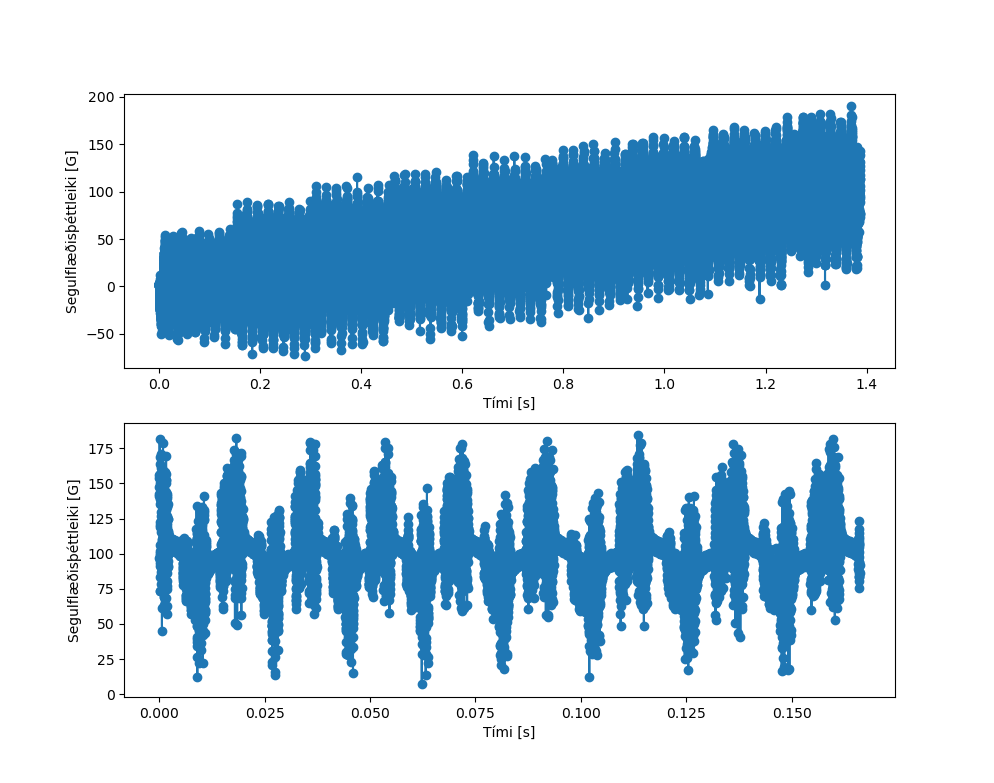
\includegraphics[width=\linewidth]{Figure_1.png}
\end{figure}
\end{document}
